\documentclass{acmart}   
\usepackage[utf8]{inputenc} 
\usepackage[greek , english]{babel}
\usepackage{alphabeta}
\usepackage{hyperref} 
\usepackage{listings}
\usepackage{color}
\usepackage{float}
\graphicspath{{./img/}}
\definecolor{mygreen}{rgb}{0,0.6,0}
\definecolor{mygray}{rgb}{0.5,0.5,0.5}
\definecolor{mymauve}{rgb}{0.58,0,0.82}

\begin{document}
       \begin{titlepage}
              \begin{center}
              \vspace*{1cm}

              \line(1,0){\textwidth}\\
              \textbf{Πρότζεκτ Ομάδας 22}\\
              \vspace{0.5cm}
              ΙΣΤΟΣΕΛΊΔΑ ΚΡΑΤΉΣΕΩΝ
              \vspace{1.5cm}
              \line(1,0){\textwidth}\\
              \textbf{Κόντος Παναγιώτης}\\
              Τμήμα: Ηλεκτρολόγων Μηχανικών \& Τεχνολογίας Υπολογιστών\\
              Τομέας: Υπολογιστές\\
              ΑΜ: 1066620\\
              Έτος Φοίτησης: 4ο\\
              \vspace{0.8cm}
              \textbf{Κωνσταντίνος Κωνσταντόπουλος}\\
                     Τμήμα: Ηλεκτρολόγων Μηχανικών \& Τεχνολογίας Υπολογιστών\\
              Τομέας: Υπολογιστές\\
              ΑΜ: 1066546\\
              Έτος Φοίτησης: 4ο\\

              \vspace{0.8cm}

              % \includegraphics[width=0.4\textwidth]{university}

              
              \end{center}
       \end{titlepage}
\tableofcontents
\newpage
\section{Εισαγωγή}
Το πρότζεκτ που μας ανατέθηκε ήταν να φτιάξουμε μια ιστοσελίδα για κρατήσεις εκδηλώσεων. 
Οι εκδηλώσεις αυτές φιλοξενούνται απο πολλους φορείς. Στην δική μας υλοποίηση ο κάθε φορέας 
θα διαθέτει εναν λογαριασμό διαχειριστή τον οποίο εισάγουμε εμείς χειροκίνητα στο σύστημα. 
Ο κάθε φορέας μπορεί να δει όλες τις εκδηλώσεις αλλα μπορεί να επεξεργαστεί μόνο τις δικές του. 
Οι χρήστες της ιστοσελίδας βλέπουν τις παραστάσεις και μπορούν να κάνουν την κράτηση που τους ενδιαφέρει.  

\section{Μεθοδολογια}
\subsection{Στόχος}
Ο κύριος στόχος μας ήταν η δημιουργία μιας ιστοσελίδας στην οποια θα υπάρχουν συγκεντρωμένες όλες 
οι εκδηλώσεις ώστε να μπορεί όποιος επιθυμεί να κλείσει εύκολα και γρήγορα θέση για την παράσταση 
της αρεσκείας του. Επιπροσθέτως η διαχείριση των εκδηλώσεων απο τους διαχειριστές θα έπρεπε να είναι 
εύκολη και να μην απαιτούνται ειδικές γνώσεις για την χρήση της ιστοσελίδας.

\subsection{Υλοποίηση}
\subsection*{Προσέγγιση}
Όταν μας ανατέθηκε το θέμα της εργασίας κανονίσαμε μία συνάντηση με τον κ. Σιντόρη ώστε να μας 
καθοδηγήσει σχετικά με τις δυνατότητες που θα παρέχει η ιστοσελίδα μας. Αφου επισκεφθήκαμε και 
ιστοσελίδες για να δούμε τον τρόπο λειτουργίας τους ξεκινήσαμε να εργαζόμαστε. Επειδή θα ήταν 
πιο δύσκολη η διεκπεραίωση της εργασίας αν δουλεύαμε στο ίδιο κομμάτι, ο ένας ασχολήθηκε πιο πολυ 
με το front-end και ο αλλος με το back-end.

\subsection*{Εργαλεία και Τεχνολογίες}
Για την δημιουργία του front end χρησιμοποιήθηκαν τα παρακάτω εργαλεία:
\begin{itemize}
       \item Handlebars
       \item CSS3
       \item Javascript
\end{itemize}
To handlebars χρησιμοποιήθηκε ώστε να μπορούμε να χρησιμοποιούμε κάποια templates και να δημιουργούμε 
δυναμικά τα html documents που σερβίρουμε στον χρήστη.
Για την δημιουργία του back end χρησιμοποιήθηκαν τα παρακάτω εργαλεία:
\begin{itemize}
       \item Node.js
       \item Express
       \item sqlite
       \item Javascript
\end{itemize}


\subsection*{Χρονοδιάγραμμα}
Αρχικά ασχοληθήκαμε με το διάγραμμα οντοτήτων-συσχετίσεων που μας ήταν γνωστό απο το μάθημα των Βάσεων Δεδομένων.
Έπειτα ξεκινήσαμε με το να σχεδιάσουμε στο χαρτί ένα προσχέδιο της ιστοσελίδας μας. 
Με την πάροδο των μαθημάτων και την απόκτηση των απαιτούμενων γνώσεων κατασκευάζαμε βήμα βήμα το front-end. 
Την τελευταία εβδομάδα που μάθαμε και για τον προγραμματισμό της ιστοσελίδας ενώσαμε τα μέρη της ιστοσελίδας μας, 
ωστε να είναι λειτουργική.

\subsection*{Δημιουργια erd και βασης δεδομένων}
Δημιουργήσαμε το διάγραμμα οντοτήτων - συσχετίσεων για τον μικροκοσμο που μας απασχολούσε όπως φαίνεται 
στην εικόνα \ref{fig:diagram}.
\begin{figure}[H]
       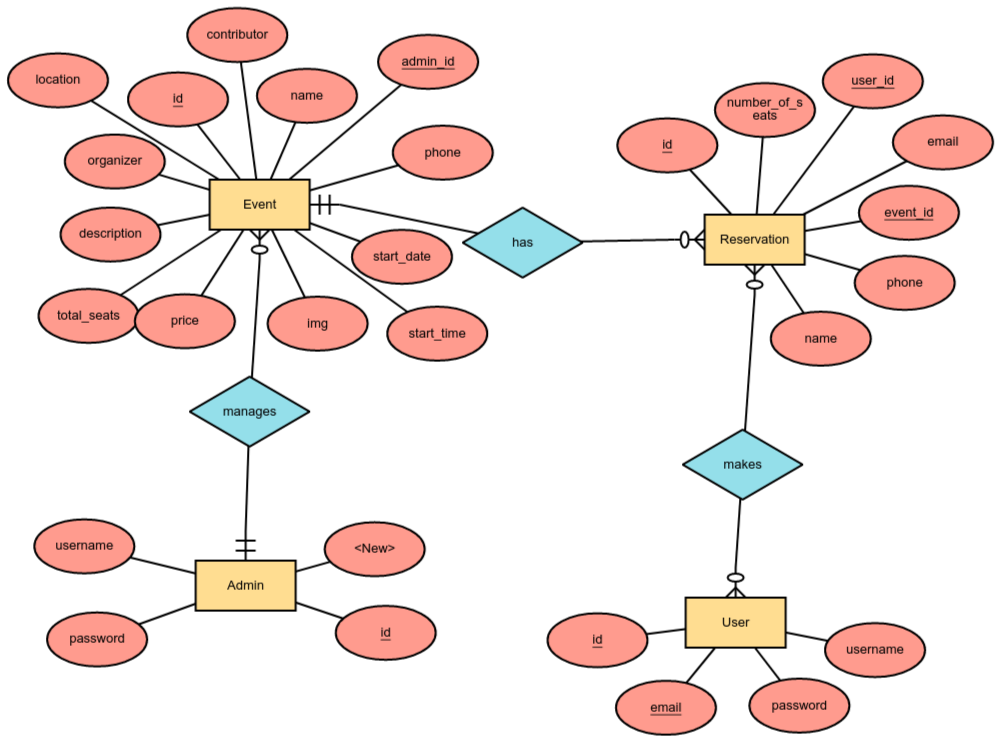
\includegraphics[width=0.5\textwidth]{diagram.png}
       \caption{Διάγραμμα οντοτήτων - συσχετίσεων}
       \label{fig:diagram}
\end{figure}
Επίσης δημιουργήσαμε την βάση δεδομένων όπου θα αποθηκεύονται και θα αντλούνται οι πληροφορίες 
που χρειαζόμαστε. Στην βάση δέν βάλαμε πολλές εκδηλώσεις, καθώς αυτές πρέπει να εισάγονται απο 
τον αντίστοιχο φορέα οργάνωσης.
\subsection{Front-end}
\subsection*{Δημιουργια της Αρχικής σελίδας}
Το πρώτο κομμάτι που φτιάξαμε μετά την βάση δεδομένων ήταν η αρχική σελίδα. 
Έχοντας πάρει ιδέες απο παρόμοιες ιστοσελίδες (π.χ \href{www.viva.gr}{Viva}) 
αποφασίσαμε οτι όλες οι σελίδες της ιστοσελίδας μας θα χρησιμοποιούν ένα λογότυπο 
με εναν τίτλο και ενα navigation bar με παραπομπές στην αρχική σελίδα (Αρχική), στις 
εκδηλωσεις (Εκδηλώσεις), στις πληροφορίες της σελίδας (Πληροφορίες), στον πίνακα ελέγχου 
(Πίνακας Ελέγχου) το οποίο φαίνεται μόνο αν ο συνδεδεμένος χρήστης είναι διαχειριστής, και στην είσοδο 
(Είσοδος) απο όπου μπορεί να πραγματοποιήσει είσοδο ή εγγραφή στην σελίδα. Επίσης στην αρχική σελίδα φαίνονται 
οι τρεις δημοφιλέστερες παραστάσεις σε carousel στο κέντρο της σελίδας. Δίνεται η δυνατότητα πατώντας πάνω στην 
εικόνα να κατευθυνθεί ο χρήστης στην συγκεκριμένη εκδήλωση.
\begin{figure}[H]
       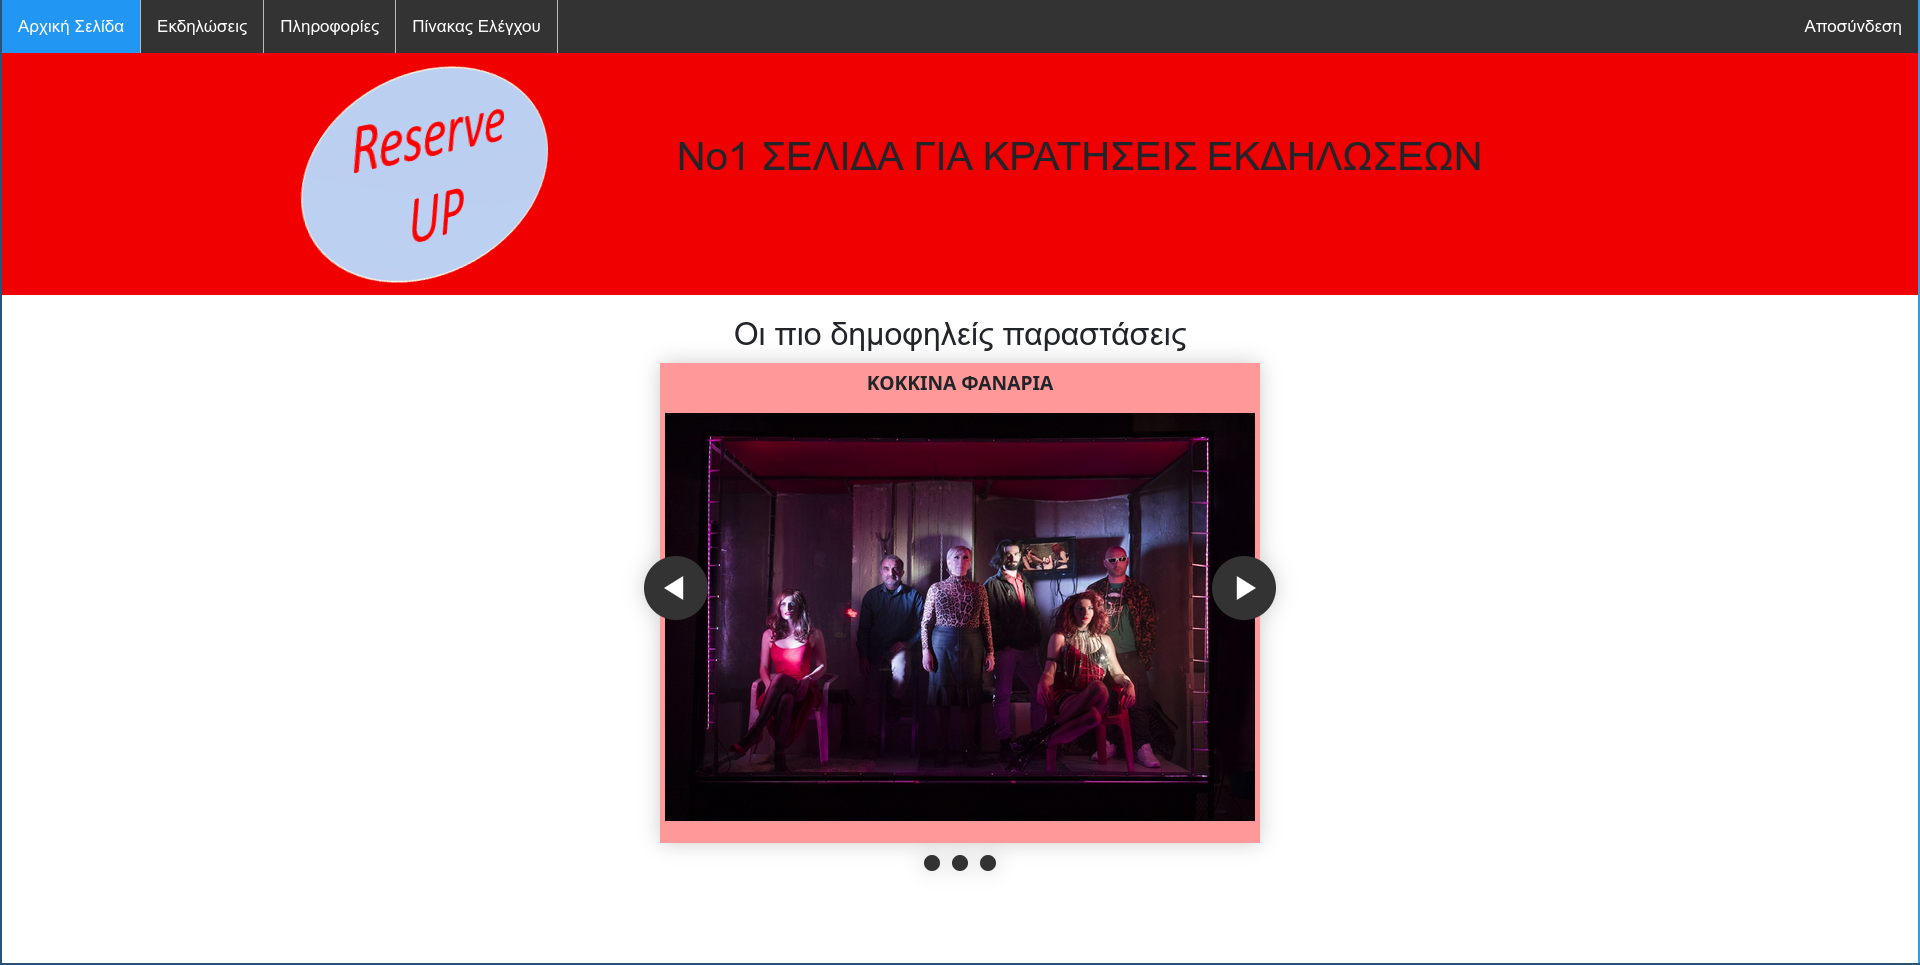
\includegraphics[width=\textwidth]{homepage.png}
       \caption{Αρχική Σελίδα}
       \label{fig:home}
\end{figure}
\subsection*{Δημιουργια της σελίδας "όλων των εκδηλώσεων"}
Στην συγκεκριμένη σελίδα φαίνονται σε μορφή λίστας όλες οι διαθέσιμες εκδηλώσεις. Υπαρχει μια μικρη 
φωτογραφία στα αριστερά, ο τίτλος, η ημερομηνία διεξαγωγής και μια μικρή περιγραφή 150 λέξεων. Πατώντας 
πάνω στην φωτογραφία, στον τίτλο ή στην ημερομηνία ο χρήστης θα μεταφερθεί στην σελίδα της εκδηλωσης.
\begin{figure}[H]
       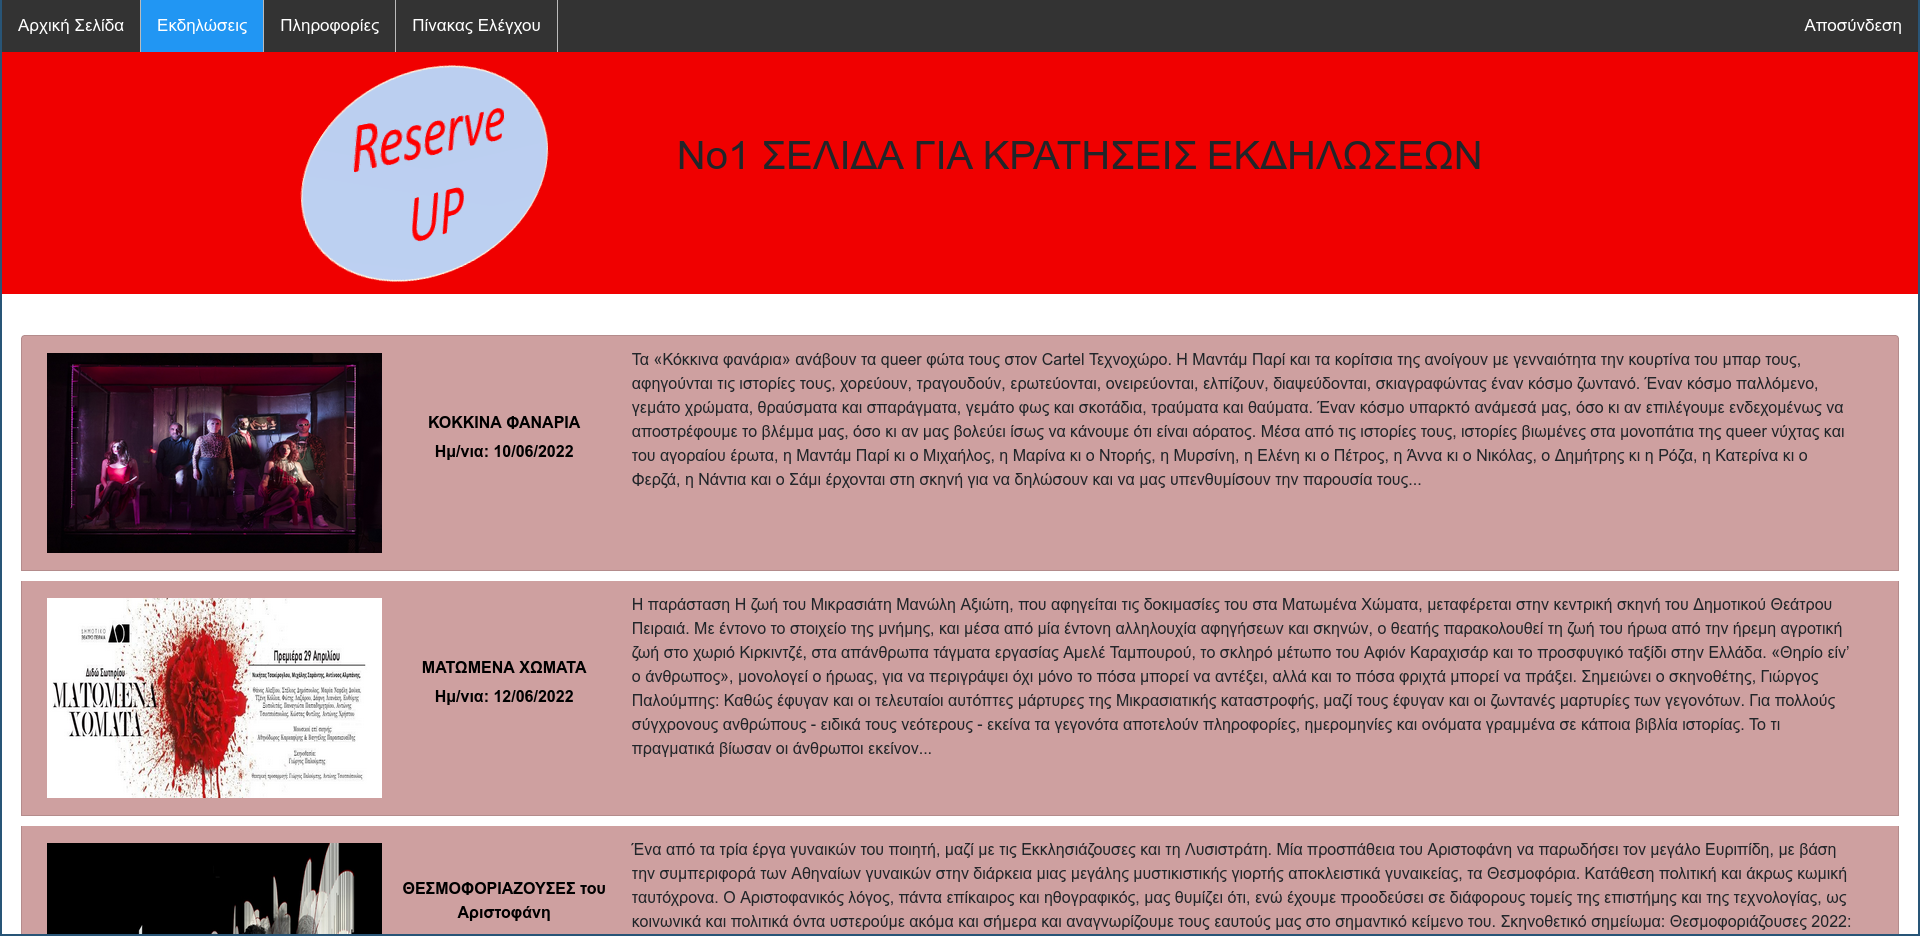
\includegraphics[width=\textwidth]{events.png}
       \caption{Λίστα Εκδηλώσεων}
       \label{fig:events}
\end{figure}
\subsection*{Δημιουργια σελίδας εκδήλωσης}
Ανοίγοντας την σελίδα της εκδήλωσης στο πάνω μέρος υπάρχει το banner της εκδήλωσης. 
Ακολουθούν ακριβως απο κάτω ο τίτλος, η ημερομηνία διεξαγωγής, το μέρος προβολής και ένα κουμπί 
για να κάνει κράτηση ο ενδιαφερόμενος χρήστης. Επιπλέον στο κάτω μέρος υπάρχει ένα μενού από το 
οποίο ο χρήστης μπορεί να επιλέξει να δει ολόκληρη την περιγραφή της παράστασης, τους συντελεστές, 
τον διοργανωτή και καποιες άλλες πληροφορίες όπως την τιμή, τις συνολικές και τις διαθέσιμες θέσεις 
και το τηλέφωνο επικοινωνίας.
\begin{figure}[H]
       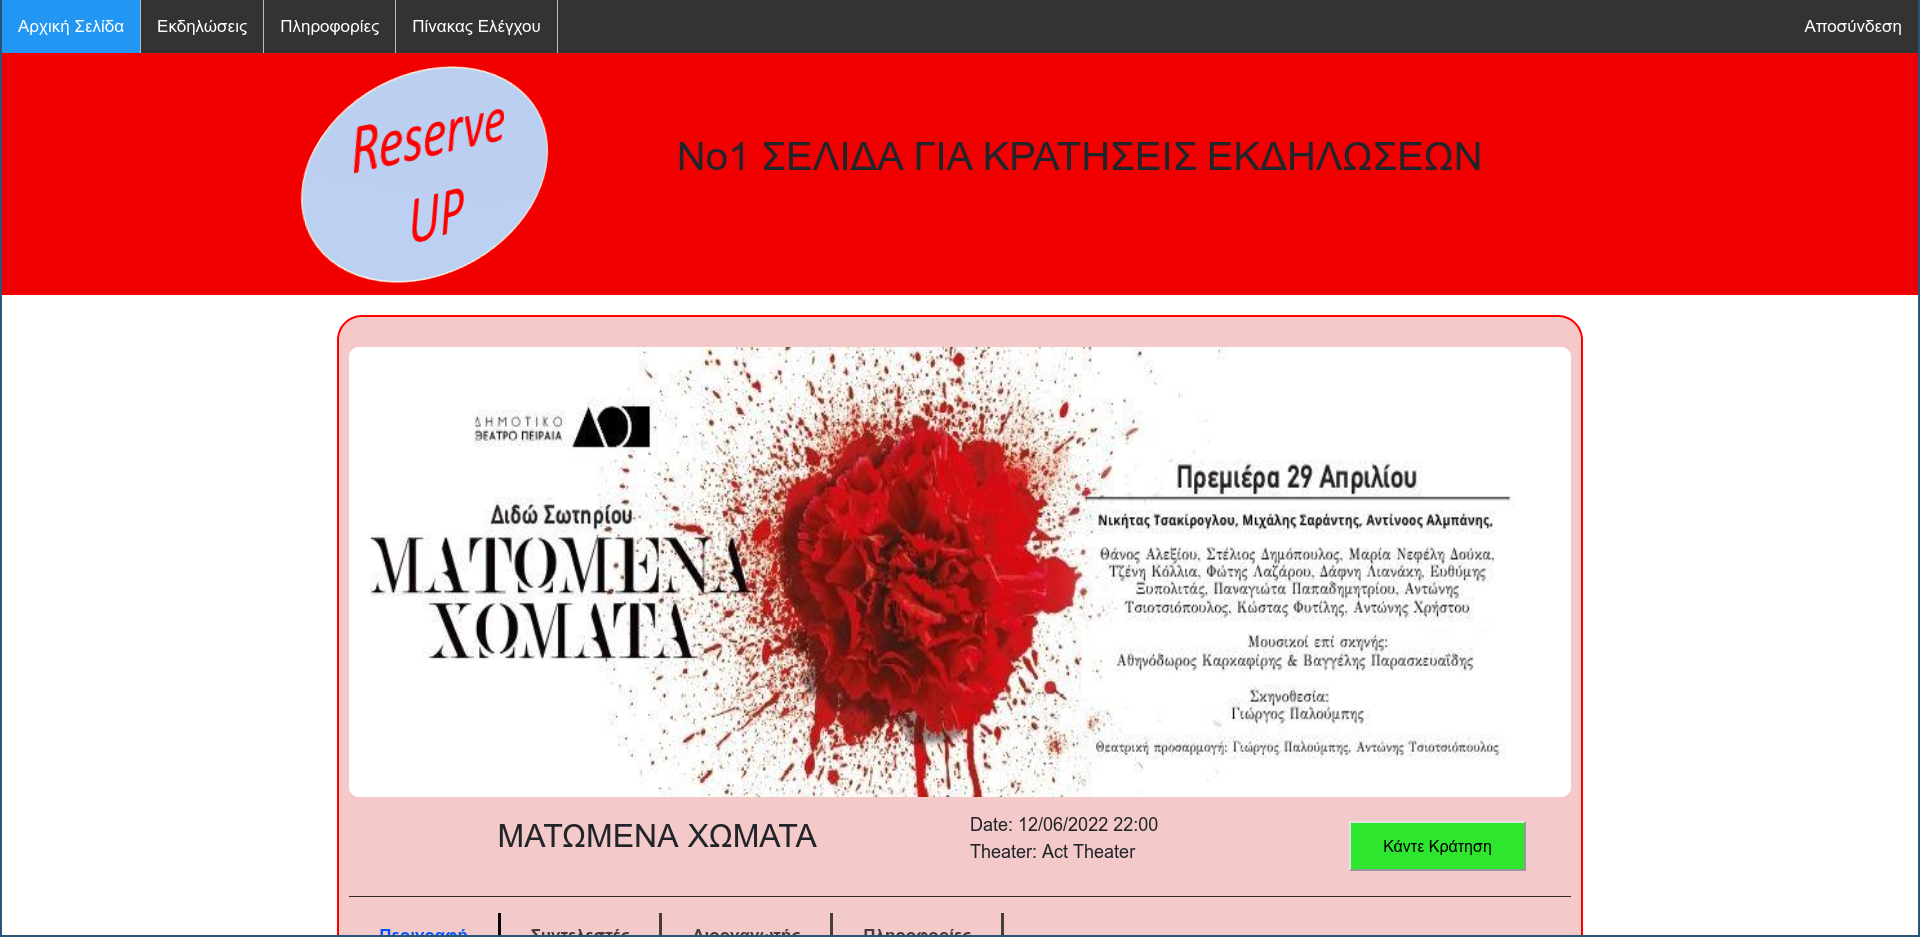
\includegraphics[width=\textwidth]{event.png}
       \caption{Σελίδα Εκδήλωσης}
       \label{fig:event}
\end{figure}
\subsection*{Δημιουργια της φόρμας κράτησης}
Εφόσον ο χρήστης επέλεξε να κάνει κράτηση πατώντας το αντίστοιχο κουμπί στην σελίδα της εκδήλωσης, 
παραπέμπεται στην φόρμα κράτησης. Τα στοιχεία που θα του ζητηθούν είναι το όνομα του, ενα email και 
ενα τηλέφωνο επικοινωνίας. Κατόπιν επιλέγει το πλήθος και τον τύπο των εισιτηρίων που επιθυμεί και στα 
δεξιά θα του εμφανιστεί το συνολικό κόστος των εισιτηρίων. Για να καταχωρηθεί η κράτηση του θα πρέπει να 
πατήσει το κουμπί "Ολοκλήρωση Κράτησης". Σε περίπτωση που δεν θέλει να συνεχίσει με την κράτηση, επιλέγοντας
ακύρωση γυρνάει στην σελίδα της εκδήλωσης.
\begin{figure}[H]
       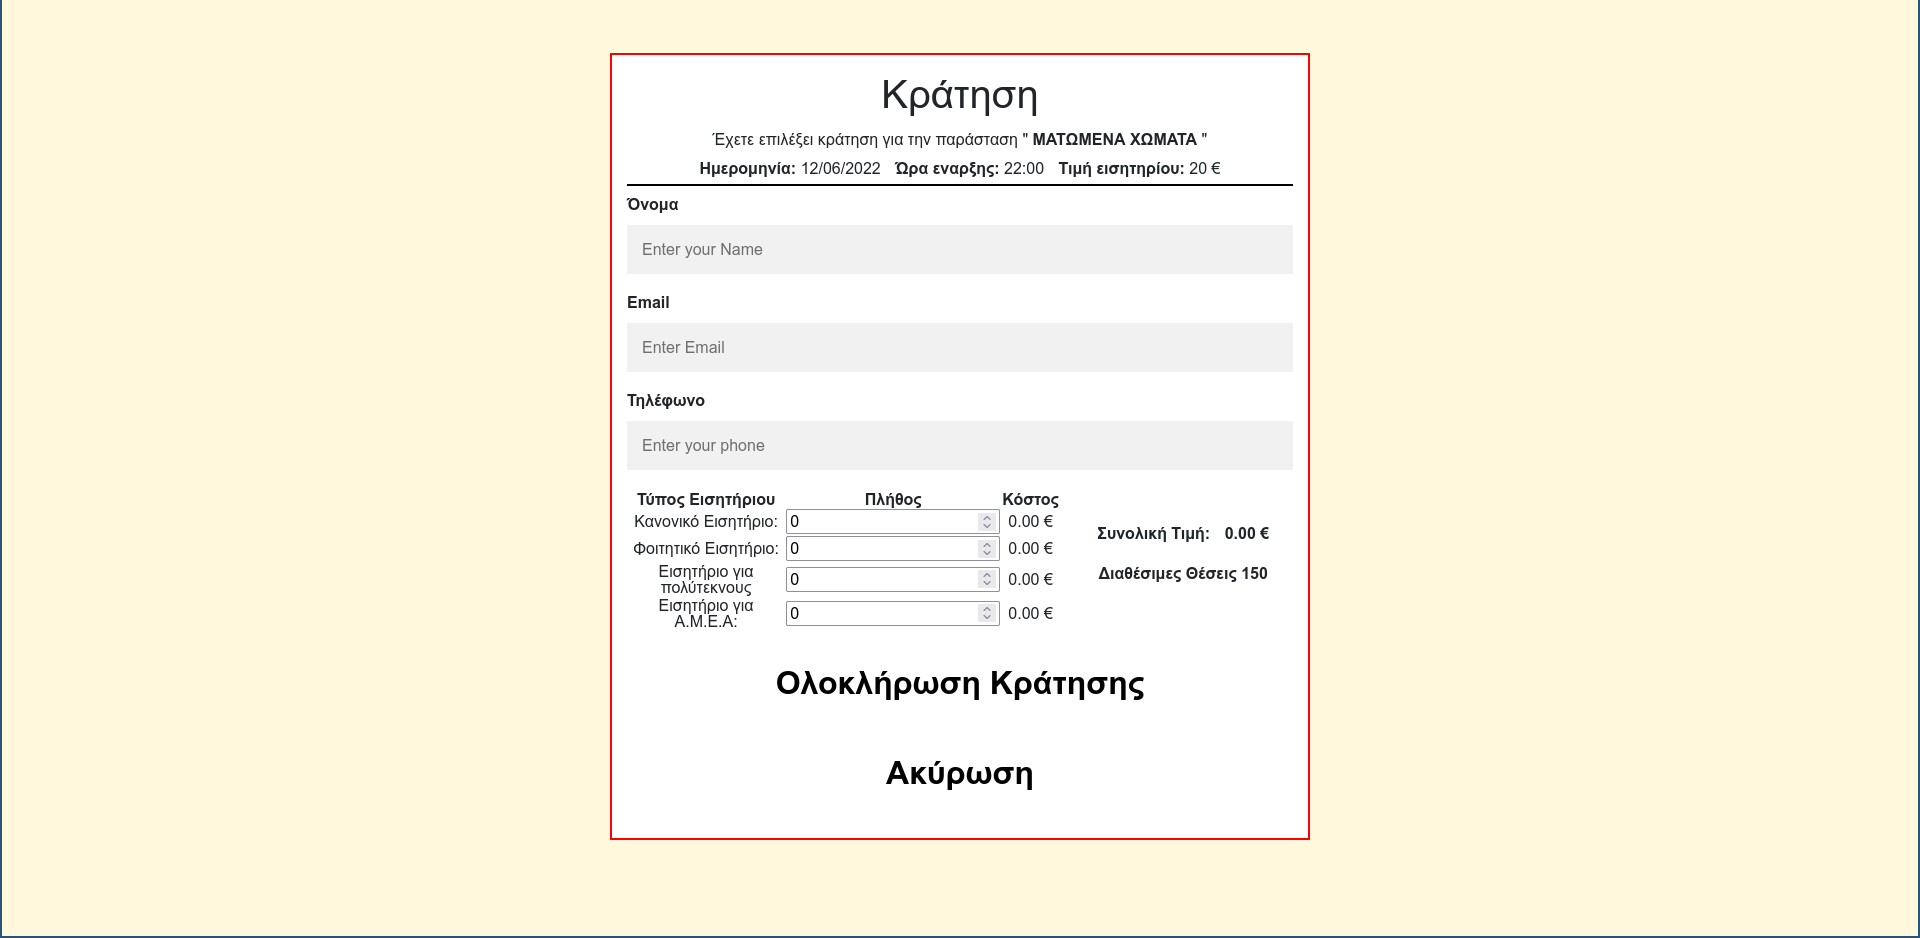
\includegraphics[width=\textwidth]{reserve.png}
       \caption{Κράτηση Εισιτηρίων}
       \label{fig:reserve}
\end{figure}
\subsection*{Δημιουργια της σελίδας Πληροφορίες}
Στην συγκεκριμένη σελίδα υπάρχουν πληροφορίες σχετικά με την λειτουργία της ιστοσελίδας και 
τους δημιουργους της. Υπαρχει ενα μενού όπου επιλέγοντας "Διαχειριστής" ή "Χρήστης" φαίνονται 
οι δυνατότητες του διαχειριστή και του απλού χρήστη αντίστοιχα.
\begin{figure}[H]
       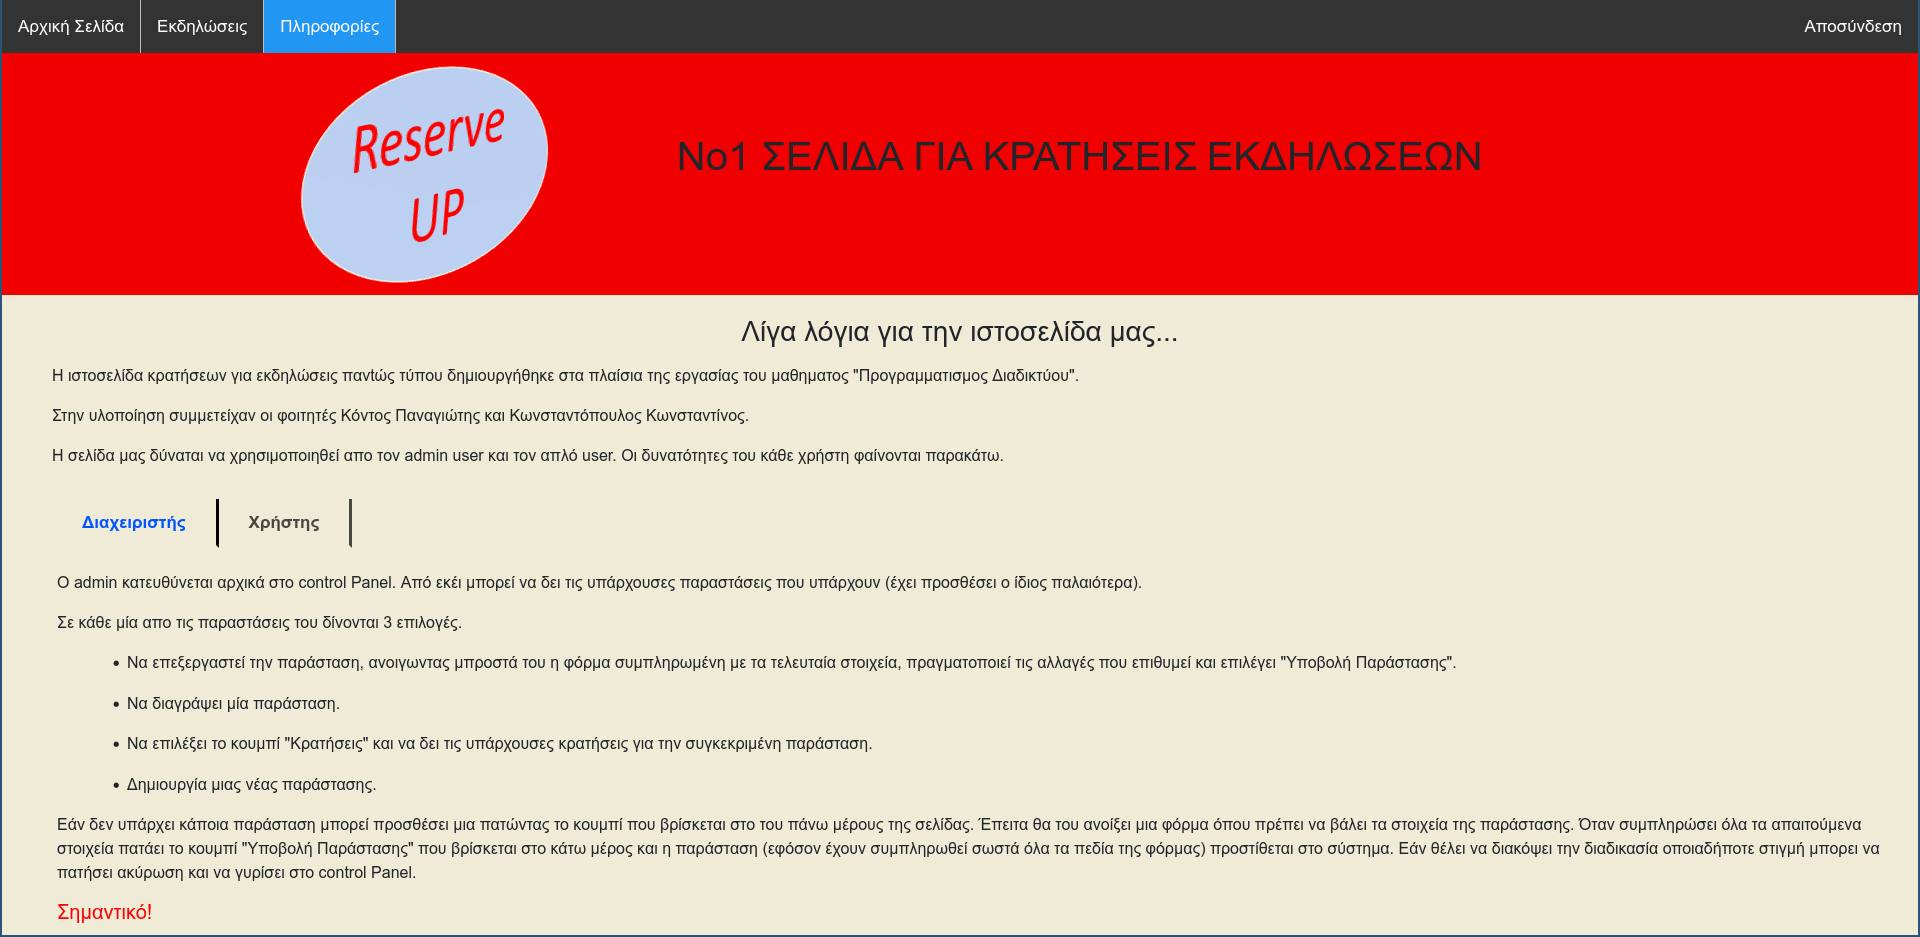
\includegraphics[width=\textwidth]{about.png}
       \caption{Σελίδα Πληροφοριων για την Ιστοσελίδα}
       \label{fig:about}
\end{figure}
\subsection*{Δημιουργια της σελίδας του Πίνακα Ελέγχου}
Εφόσον ο χρήστης που θα συνδεθεί είναι διαχειριστής, θα του εμφανιστεί ο πίνακας ελέγχου.
Εκεί μπορεί να δεί όσες εκδηλώσεις έχει προσθέσει ο ίδιος παλαιότερα. Στις συγκεκριμένες 
εκδηλώσεις έχει τρεις επιλογές.
\begin{itemize}
  \item Επεξεργασία, όπου πατώντας το κουμπί του ανοίγει η φόρμα της εκδήλωσης συμπληρωμένη με 
  τα τελευταία στοιχεια που είχε εκχωρήσει. Μπορεί να πραγματοποιήσει τις αλλαγές που επιθυμεί 
  και πατώντας "Αποθήκευση Παράστασης" ή να επιλέξει ακύρωση και θα ανακατευθυνθεί πίσω στον 
  πίνακα ελέγχου και μπορεί να δεί τις αλλαγες εφόσον τις πραγματοποίησε. 
  \item Διαγραφή, όπου σβήνει απο την βάση την συγκεκριμένη εκδήλωση.
  \item Κρατήσεις, όπου θα του ανοίξει μια νέα σελίδα και θα δει σε έναν πίνακα τις 
  υπάρχουσες κρατήσεις και τα στοιχεία τους.
\end{itemize}
Επιπροσθέτως μπορεί να κάνει "Δημιουργία" μιας νέας εκδήλωσης πατώντας στο κουμπί που 
βρίσκεται στο πάνω μέρος της οθόνης.
\begin{figure}[H]
       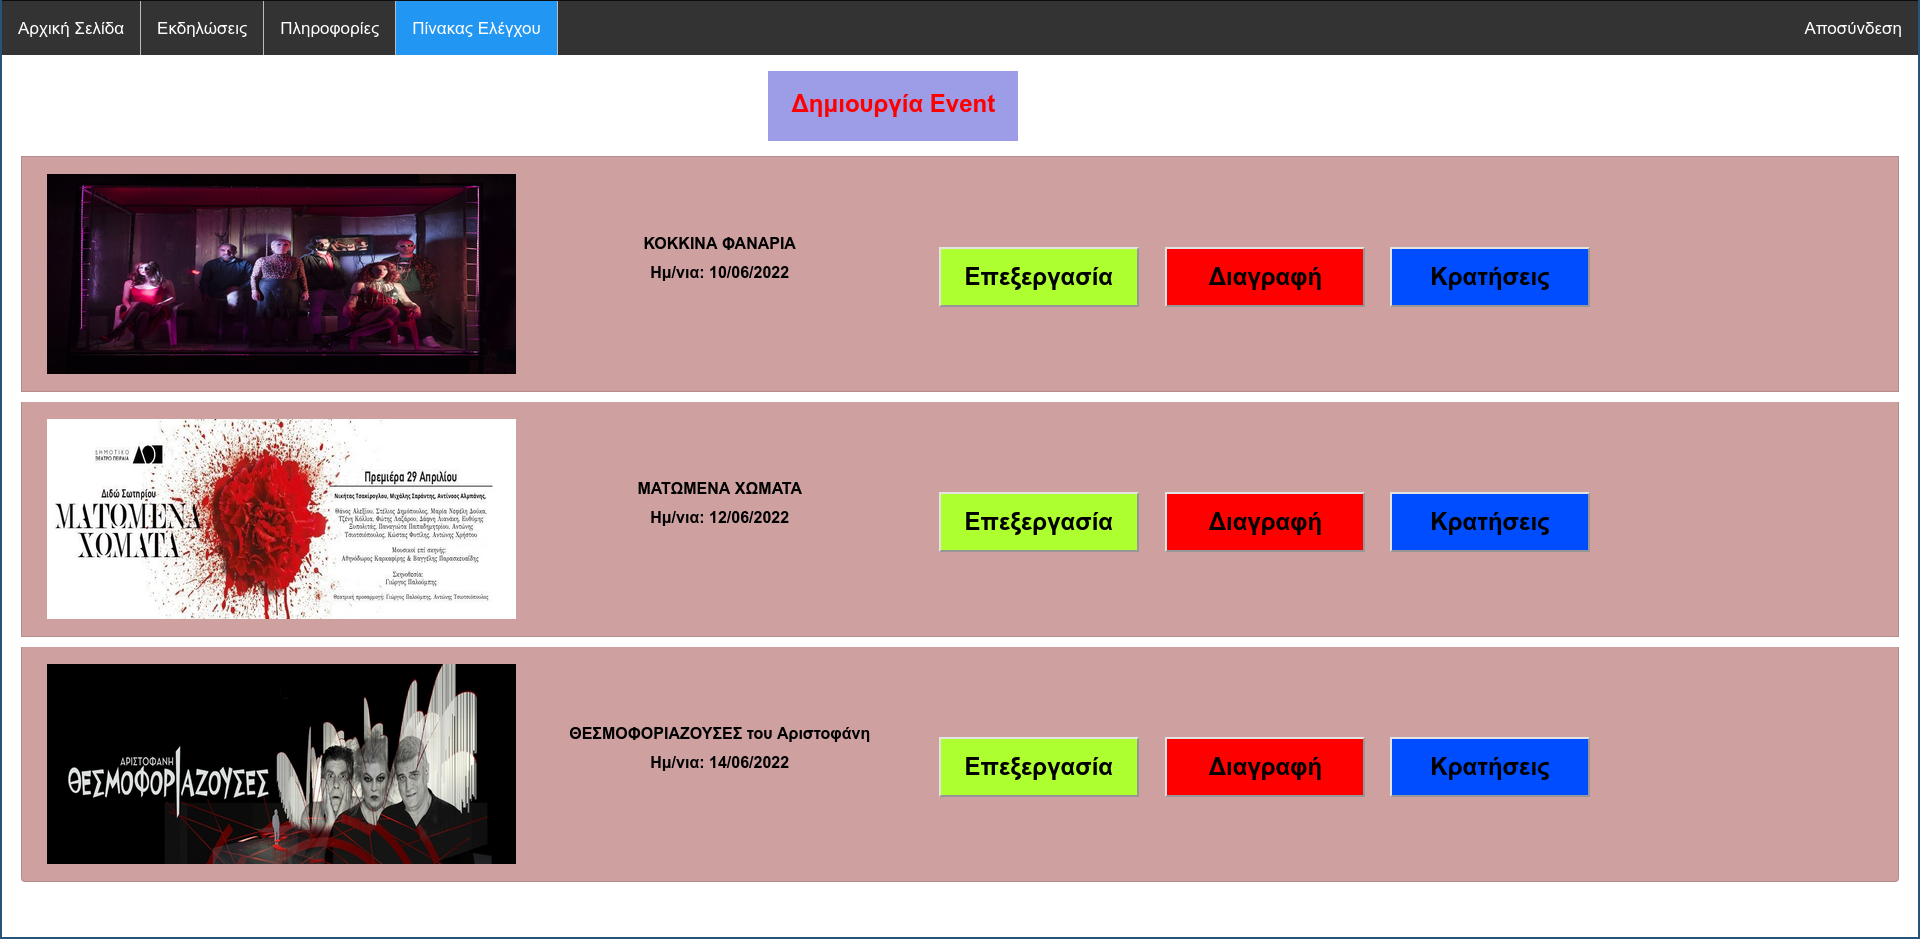
\includegraphics[width=\textwidth]{control.png}
       \caption{Πίνακας Ελέγχου}
       \label{fig:control}
\end{figure}
\subsection*{Δημιουργια της φόρμας Εκδήλωσης}
Αφού ο διαχειριστής επέλεξε να δημιουργήσει μια νέα εκδήλωση, του εμφανίζεται η φόρμα της εκδήλωσης. 
Εκεί πρέπει να εισάγει τα απαραίτητα στοιχεία και έαν θέλει την περιγραφή και τους συντελεστές. 
Εφόσον επιλέξει "Υποβολή Παράστασης" αυτή θα καταχωρηθεί στο σύστημα και θα ανακατευθυνθει πίσω 
στον πίνακα ελέγχου. Εάν επιλέξει ακύρωση, θα επιστρέψει πίσω στο πίνακα ελέγχου χωρίς καμία αλλαγή.
\begin{figure}[H]
       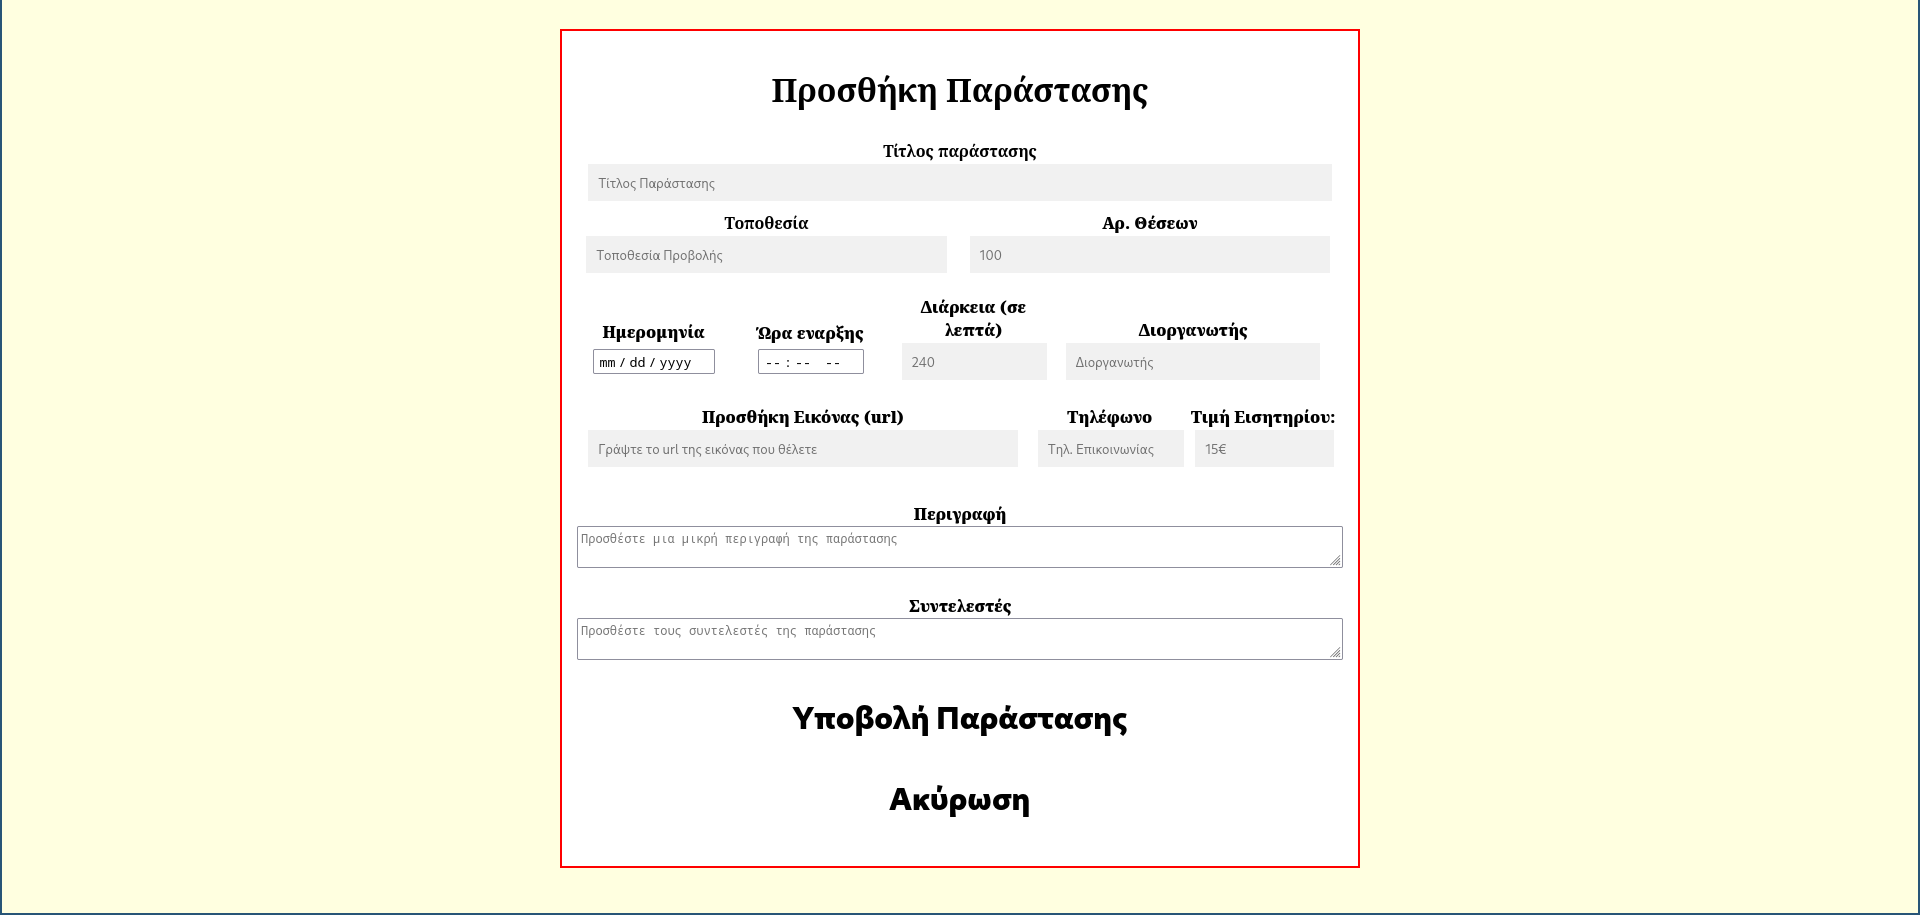
\includegraphics[width=\textwidth]{edit.png}
       \caption{Προσθήκη ή Επεξεργασία Εκδήλωσης}
       \label{fig:edit}
\end{figure}
\subsection{Back-end}
\subsection*{Δημιουργία Βάσης Δεδομένων}
Αφού έχουμε κάνει τον σχεδιασμό της βάσης, αρχικά αποφασίσαμε χρησιμοποιήσουμε sqlite για την διαχείριση της βάσης καθώς
είμαστε πιο εξοικειωμένη με αυτήν.
Δημιουργήσαμε ένα αρχείο database.sql το οποίο περιέχει τις εντολές που χρειάζονται για να δημιουργήσουμε τη βάση.
Για να γεμίσουμε την βάση με ενδεικτικές τιμές δημιουργήσαμε ένα script (populateDb.js) το οποίο αρχικά τρέχει το αρχείο
database.sql και στην συνέχεια κάνει insert στην βάση που μόλις δημιούργησε κάποιες εγγραφές.
Συγκεκριμένα εισάγει δύο διαχειριστές , τρεις απλους χρήστες και πέντε εκδηλώσεις.
Αφού δημιουργήσαμε την βάση, χρειάστηκε να φτιάξουμε ένα model.js το οποίο περιέχει όλες συναρτήσεις που χρειάζονται
για να αντλήσουμε και να εισάγουμε στοιχεία από τη βάση.
\subsection*{Session}
Για να μπορούμε να ελέγχουμε άμα ο χρήστης είναι συνδεδεμένος και τι είδος χρήστη είναι χρησιμοποιήσαμε την βιβλιοθήκη
express-session με την οποία ορίσαμε το cookies και μπορούσαμε να ελέγχουμε αν ο χρήστης είναι συνδεδεμένος ή όχι και 
είδος χρήστη είναι (διαχειριστής ή απλός).
Αφού δημιουργηθεί μια επιτυχής σύνδεση μπορούμε τότε να ορίσουμε τις μεταβλητές 
\begin{lstlisting}
req.session.userId = user.id
\end{lstlisting}
και
\begin{lstlisting}
req.session.userType = user.type
\end{lstlisting}
Με αυτόν τον τρόπο μπορούμε να βλέπουμε στο session τα χαρακτηριστικά του συνδεδεμένου χρήστη.
\subsection*{Routes}
Στο directory routes του πρότζεκτ υπάρχουν όλα τα αρχεία που είναι υπεύθυνα για όλες τις διαθέσιμες διαδρομές 
και το τι πρέπει να γίνει ανάλογα με τη διαδρομή που επιλέγει ο χρήστης.
Στο index.js ορίζουμε τον router για τον root της σελίδας μας και ορίζουμε επίσης σε ποια αρχεία πρέπει να αναφέρεται
όταν αλλάζει η διαδρομή.
Συγκεκριμένα το setup των routes, όπως είναι ορισμένα στο index.js, φαίνεται παρακάτω:
\begin{lstlisting}
const router = express.Router();

const loginRouter = require('./login.js');
const eventRouter = require('./event.js');
const formRouter = require('./form.js');
const aboutRouter = require('./about.js');
const eventFormRouter = require('./eventForm.js');
const eventsRouter = require('./events.js');
const controlPanelRouter = require('./controlPanel.js');
const reservationsRouter = require('./reservations.js');

router.use((req, res, next) => {
       next();
});

//Rest Routes
router.use('/login', loginRouter);
router.use('/event', eventRouter);
router.use('/form', formRouter);
router.use('/about', aboutRouter);
router.use('/eventForm', eventFormRouter);
router.use('/events', eventsRouter);
router.use('/controlPanel', controlPanelRouter);
router.use('/reservations', reservationsRouter);

\end{lstlisting}

Και παρακάτω φαίνεται πως είναι ένα αρχείο router:
\begin{lstlisting}
const express = require('express');
const controller = require('../controllers/controlPanel');
const loginController = require('../controllers/login');
const router = express.Router();

router.use((req, res, next) => {
       next();
});

router.get('/', loginController.checkAuthenticated, loginController.checkAdmin, 
controller.getEventsByAdminId);
router.get('/delete/:id', loginController.checkAuthenticated, loginController.checkAdmin, 
controller.deleteEvent);
router.get('/edit/:id', loginController.checkAuthenticated, loginController.checkAdmin, 
controller.getEditById);
router.get('/reservations/:id', loginController.checkAuthenticated, 
loginController.checkAdmin, controller.getReservationsById);
router.post('/update/:id', loginController.checkAuthenticated, loginController.checkAdmin, 
 controller.updateEvent);

module.exports = router;
\end{lstlisting}

\subsection*{Controllers}
Στο directory Controllers υπάρχουν τα αρχεία τα οποίο περιέχουν τις συναρτήσεις που καλούνται αντίστοιχα απο τον κάθε
router. Ένας τέτοιος controller είναι ο login, ο οποίος περιέχει της συναρτήσεις που ελέγχουν αν ο χρήστης είναι 
συνδεμένος ή όχι και αν είναι διαχειριστής ή απλός χρήστης. Παρόμοια έχουν δημιουργηθεί και οι άλλοι controllers, δηλαδή
περιέχουν συναρτήσεις που χρειάζονται ανάλογα με την διαδρομή που έχει επιλεχθεί.
Στις περιπτώσεις που ο controller χρειάζεται να επικοινωνήσει με τη βάση, τότε χρησιμοποιούνται οι συναρτήσεις που υπάρχουν 
στο model.js και ο controller περιμένει απάντηση απο την βάση.

<<<<<<< HEAD
\section{Οδηγίεσ χρήσησ και εγκατάστασησ τησ εφαρμογησ}
Το πρόξεκτ μπορεί να βρεθεί στο \href{https://github.com/KonstantoJr/web_dev_project}{Github}.
=======
\section{Λειτουργία ΕφαρμογήΣ}
Το πρότζεκτ μπορεί να βρεθεί στο \href{https://github.com/KonstantoJr/web_dev_project}{Github}.
>>>>>>> c9def4825b6fd6f4955d9598b5444fc4894b53ce
Αρχικά, χρειάζεται να δημιουργήσουμε το αρχείο της βάσης μας, για να γίνει αυτό πρέπει από το root directory
του πρότζεκτ να μεταφερθούμε στο /model/sqlite και να τρέξουμε την εντολή 
\begin{lstlisting}
node populateDb.js 
\end{lstlisting}
Αυτό θα δημιουργήσει το αρχείο της βάσης και θα γεμίσει την βάση με ενδεικτικά δεδομένα.
Για να δοκιμάσετε την λειτουργία του admin μπορείτε να χρησιμοποιήσετε τον λογαριασμό 
\begin{itemize}
       \item username: admin password: admin
       \item username: theater password: theater
\end{itemize}
Καθώς ο admin δεν γίνεται να κάνει register από την ιστοσελίδα και χρειάζεται να εισαχθεί στην βάση από τους 
διαχειριστές του σέρβερ.
Για την λειτουργία του χρήση μπορείτε είτε να δημιουργήσετε καινούργιο , είτε να χρησιμοποιήσετε έναν υπάρχον.
\begin{itemize}
       \item username: user1 password: user1
       \item username: user2 password: user2
       \item username: user3 password: user3     
\end{itemize}
Να σημειωθεί πως οι κωδικοί στην βάση είναι κρυπτογραφημένοι.

Στην συνέχεια αφού ετοιμάσουμε την βάση επιστρέφουμε στο root directory και τρέχουμε την εντολή:
\begin{lstlisting}
       npm install -y 
\end{lstlisting}
για να κατεβάσουμε τα modules που χρειάζονται για την λειτουργία της εφαρμογής.
Στην συνέχεια εκτελούμε την εντολή:
\begin{lstlisting}
       npm run debug
\end{lstlisting}
Και πλέον μπορούμε να πάμε στο \url{http://localhost:3000/} και να δούμε την εφαρμογή.


\section{Λειτουργία Εφαρμογής}
Η σελίδα μας δύναται να χρησιμοποιηθεί απο τον admin user και τον απλό user. Οι δυνατότητες του κάθε χρήστη φαίνονται παρακάτω.

\subsection{Διαχειρηστής}
Ο admin κατευθύνεται αρχικά στο control Panel. Από εκέι μπορεί να δει τις υπάρχουσες παραστάσεις που υπάρχουν (έχει προσθέσει ο ίδιος παλαιότερα).

Σε κάθε μία απο τις παραστάσεις του δίνονται 3 επιλογές.
\begin{itemize}
\item Να επεξεργαστεί την παράσταση, ανοιγωντας μπροστά του η φόρμα συμπληρωμένη με τα τελευταία στοιχεία, πραγματοποιεί τις αλλαγές που επιθυμεί και επιλέγει "Υποβολή Παράστασης".

\item Να διαγράψει μία παράσταση.

\item Να επιλέξει το κουμπί "Κρατήσεις" και να δει τις υπάρχουσες κρατήσεις για την συγκεκριμένη παράσταση.

\item Δημιουργία μιας νέας παράστασης.
\end{itemize}

Εάν δεν υπάρχει κάποια παράσταση μπορεί προσθέσει μια πατώντας το κουμπί που βρίσκεται στο του πάνω μέρους της σελίδας. Έπειτα θα του ανοίξει μια φόρμα όπου πρέπει να βάλει τα στοιχεία της παράστασης. Όταν συμπληρώσει όλα τα απαιτούμενα στοιχεία πατάει το κουμπί "Υποβολή Παράστασης" που βρίσκεται στο κάτω μέρος και η παράσταση (εφόσον έχουν συμπληρωθεί σωστά όλα τα πεδία της φόρμας) προστίθεται στο σύστημα. Εάν θέλει να διακόψει την διαδικασία οποιαδήποτε στιγμή μπορει να πατήσει ακύρωση και να γυρίσει στο control Panel.

\subsection{Απλός χρήστης}

\begin{itemize}

\item Ο απλός user έχει πρόσβαση στην αρχική σελίδα όπου βλέπει τις 3 δημοφιλέστερες παραστάσεις την τρέχουσα στιγμή. Πατώντας πάνω στην εικόνα θα κατευθυνθεί στην σελίδα της συγκεκριμένης παράστασης.

\item Να επιλέξει απο το menu στο πάνω μέρος να δεί όλα τα events που είναι διαθέσιμα. Υπάρχει η εικόνα της παράστασης, ο τίτλος, η ημερομηνία και μια μικρή περιγραφή που έχει προστεθεί απο τον διοργανωτή. Απο εκεί πατώντας πάνω σε κάποιο event θα ανακατευθυνθεί στην αντίστοιχη σελίδα με τις πληροφορίες του event.

\item Στην σελίδα με τις πληροφορίες της παράστασης φαίνονται αναλυτικά όλα τα στοιχεία. Πατώντας στο κουμπί που υπάρχει στα δεξιά "Κάντε Κράτηση" θα του ανοίξει μία φόρμα για να συμπληρώσει τα στοιχεία του και τα εισητήρια που επιθυμεί. Εαν δεν έχει κάνει κάποιο λάθος στην συμπήρωση της φόρμας, μόλις πατήσει "Ολοκλήρωση Κράτησης" στο κάτω μέρος θα ανακατευθυνθεί στην σελίδα της παράστασης και θα του εμφανιστεί μήνυμα ότι η κράτηση καταχωρήθηκε επιτυχώς!
\end{itemize}


\end{document}